\chapter{Mitigazione degli attacchi}


\section{Introduzione}

Mitigare gli attacchi DDoS è un problema di più difficile risoluzione rispetto alla sola rilevazione, perchè bisogna conoscere maggiori informazioni sulla provenienza del flusso malevolo e il problema dei ``false positive'' è maggiormente sentito: se durante la fase di detection rileviamo un falso positivo e lo notifichiamo all'amministratore di sistema \underline{non è un grande problema} perchè sarà lui ad effettuare una successiva analisi prima di intraprendere azioni correttive. Se ci prefiggiamo l'obiettivo di bloccare automaticamente i flussi malevoli dei falsi positivi significherà degradare la connessione ad utenti legittimi.

\subsection{Ip spoofing}

L'ip spoofing è una tecnica che permette di costruire pacchetti IP con indirizzo IP sorgente modificato con lo scopo di fingersi un altro dispositivo o nascondere la propria identità.È un grande problema di sicurezza delle reti, principalmente perchè permette effettuare attacchi DDoS, permettendo di effettuare attacchi come l'amplificazione DNS oppure rendendo più difficile l'identificazione della sorgente dell'attacco nelle altre tipologie.

%todo: cite https://www.cloudflare.com/it-it/learning/ddos/glossary/ip-spoofing/


\paragraph{Bloccare l'ip spoofing}
Per mitigare questo problema abbiamo introdotto una regola iptables nel router \ref{code:iptablesrule}, la quale impedisce l'inoltro di pacchetti provenienti da sottoreti diverse da quella in cui è situato il router.
Iptables è un firewall integrato nel kernel linux.
% https://wiki.archlinux.org/title/Iptables_(Italiano)#:~:text=Iptables%20%C3%A8%20un%20potente%20firewall,%C3%A8%20usato%20per%20gli%20IPv6.

% todo: la regola è corretta?
\begin{lstlisting}[caption={Esempio di regola iptables}\label{code:iptablesrule}]
    mettere la regola qui
\end{lstlisting}
Questa soluzione impedisce solo parzialmente l'utilizzo dell'ip spoofing, perchè sarà sempre possibile generare pacchetti con ip spoofing provenienti da qualsiasi indirizzo ip della sottorete in cui si trova l'attaccante.


\section{Tool utilizzati}
Prova prova

Per mitigare un attacco devo conoscere un maggior numero di informazioni riguardo al traffico in forma non aggregata, per questa motivazione utilizzo degli ulteriori tool per raccogliere dati sui flussi transitanti per un'interfaccia in maniera non aggregata.

\subsection{Netflow}

Netflow è un software introdotto inizialmente nei router Cisco nel 1996, successivamente è stato creata un'estensione standardizzata dall'IETF, chiamata IPFIX. Netflow è uno dei tool di monitoring più famosi e permette di monitorare e registare informazioni riguardo i flussi che attraversano una determinata interfaccia.
% todo: tabella con features raccolete da netflow

% \begin{center}
%     \begin{tabular}{c c c c c}
%         IN\_BYTES & IN\_PKTS & FLOWS & PROTOCOL & SRC\_TOS \\ TCP\_FLAGS  &  L4\_SRC\_PORT & IPV4\_SRC\_ADDR & SRC\_MASK INPUT\_SNMP \\ L4\_DST\_PORT & IPV4\_DST\_ADDR



%     \end{tabular}
% \end{center}

Poichè non è possibile estendere le features di netflow e non rispecchiano completamente i nostri interessi abbiamo deciso di progettare il nostro agent utilizzando altre soluzioni.
% todo: le features di netflow le posso modificare?

\subsection{Berkley Packet Filter (BPF)}

Il Berkley Packet Filter (BPF) è una tecnologia introdotta nel kernel di alcuni sistemi operativi, tra cui il kernel linux, su cui è stata introdotta a partire dalla versione 2.1.75 del kernel, nel 1997. BPF consiste in una macchina virtuale, con una virtual cpu special purpose, integrata nel kernel, che permette il filtraggio e l'analisi dei pacchetti in transito su un'interfaccia.
È una soluzione che permette di eseguire un bytecode in maniera sicura nello spazio kernel utilizzando una sandbox ed eliminando l'overhead delle system call e del context switching tra kernel e user. 
Per effettuare il filtering tramite BPF deve essere generato del codice in un particolare assembly in grado di funzionare sulla CPU virtuale, che verrà richiamato alla ricezione di ogni pacchetto sull'interfaccia determinata (event driven). 
Un esempio del suo utilizzo è tcpdump che sfrutta BPF per effettuare il filtraggio in maniera efficiente. L'esempio di bytecode \ref{code:esempiobpf} permette di filtrare i pacchetti IPV4, per farlo verifica se l'ethertype è uguale a 0x800 \cite{risso_ebpf}.

%todo: cite https://drive.google.com/file/d/14dRWGwAJKBqB1N6-NOBHUxoeOILPYQjN/view
% https://docs.cilium.io/en/stable/bpf/

% todo: esempio tcpdump codice => vedi slide risso

\begin{lstlisting}[caption={Esempio delle istruzioni per il filtering dei pacchetti IP in BPF assembly}\label{code:esempiobpf}]
user@linux$ tcpdump -d ip
(000) ldh [12]
(001) jeq #0 x800 jt 2 jf 3
(002) ret #96
(003) ret #0
\end{lstlisting}

\subsection{extended Berkeley Packet Filter (eBPF)}
% https://docs.cilium.io/en/stable/bpf/

La extended Berkeley Packet Filter è una versione che estende la versione originale ed è stata introdotta nella versione 3.18 del kernel Linux, ai giorni nostri la versione originale è completamente obsoleta e anche il codice scritto per la vecchia versione, per esempio tcpdump, viene tradotto trasparentemente per la nuova \cite{cilium_ebpf}.

\begin{figure}[]
    % todo: capire come gestire citazioni imsmagini a livello di copyright
    %  e capire come funzionano le label per richiamare le immagini
    \label{fig:ebpf}
    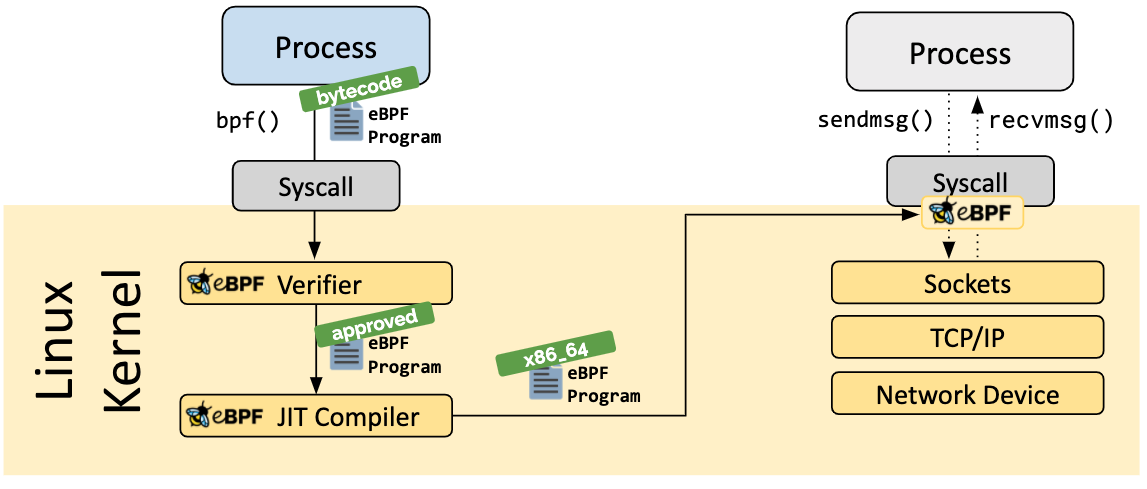
\includegraphics[width=\hsize]{images/mitigazione/ebpf_architecture.png}
    \caption{Architettura eBPF \cite{ebpf.io}.}
    \centering
\end{figure}

Prima che il bytecode sia caricato nel kernel Linux vengono effettuati due passaggi, come si può notare dall'immagine \ref{fig:ebpf}. La prima è la ``Verication'', la quale si occupa di verificare che il programma sia sicuro da eseguire e verifica che: il programma abbia lunghezza limitata, che non ci siano accessi a indirizzi di memoria non validi e che abbia una fine, di conseguenza controlla che non siano presenti cicli infiniti. 
Effettuata la verifica viene eseguita la ``Just-in-Time (JIT) compilation'', la quale traduce il bytecode generico in istruzioni specifiche per la macchina che lo sta eseguendo, questo permette di incrementare le prestazioni e rendere i programmi eBPF efficienti come i moduli kernel compilati nativamente \cite{ebpf.io}.
eBPF inoltre fornisce strumenti utili per lo sviluppo, come le mappe e gli helpers.

Le mappe sono un importante aspetto dei programmi eBPF, esse permettono di memorizzare dati in delle strutture chiave/valore in kernel space, che possono essere condivise con altri programmi eBPF oppure con applicazioni in user space \cite{cilium_ebpf}.

La chiamata di generiche funzioni a livello kernel non è consentita, sia per mantenere la compatibilità del programma non solo con una determinata versione del kernel, per questo motivo sono stati introdotti gli ``helpers'', inoltre permettono l'esecuzione di istruzioni o permettono di eseguire alcuni task non permessi dall'assembly eBPF per motivi di sicurezza.

Un ulteriore caratteristica di eBPF è la possibilità di potere concatenare l'esecuzione dei programmi, chiamandoli a cascata,in maniera simile alla ``execve()'', durante l'esecuzione.

I vantaggi di un programma eBPF rispetto alla scrittura di un modulo kernel sono molteplici: permettono l'esecuzione sicura del codice senza la possibilità che vada a corrompere il kernel, non c'è rischio che le nuovi versioni del kernel vadano a interrompere il suo funzionamento e garantisce le stesse prestazioni.

% https://ebpf.io/

\subsection{eXpress Data Path (XDP)}

Il kernel Linux supporta più punti dello stack di rete in cui è possibile agganciare l'esecuzione dei programmi eBPF.
XDP (eXpress Data Path) è un hook ad alte performance che permette di eseguire un programma eBPF al primo punto possibile, questo permette grandi performance, perchè il processamento avviene prima che qualsiasi altro processamento possa avvenire. XDP è un punto d'aggancio ideale per il filtering dei pacchetti malevoli o inaspettati e in qualsiasi comune protezione anti DDoS \cite{cilium_xdp}.
Il programma inserito su un hook XDP può compiere cinque azioni possibili:
\begin{itemize}
    \item XDP\_PASS: lascia passare il pacchetto nel normale stack di rete
    \item XDP\_DROP: ignora semplicemente il pacchetto, senza compiere ulteriori azioni
    \item XDP\_TX, restituisce il pacchetto alla stessa interfaccia, normalmente modificato
    \item XDP\_ABORTED: è un valore di ritorno che il programmatore non dovrebbe utilizzare, segnala un che si è verificato un errore nel programma eBPF, per esempio una divisione per zero e contemporaneamente ignora il pacchetto come l'XDP\_DROP
    \item XDP\_REDIRECT: reindirizza il pacchetto verso un'altra scheda di rete, o in user space
\end{itemize}
\begin{figure}[]
    % todo: capire come gestire citazioni imsmagini a livello di copyright
    % https://www.researchgate.net/publication/333998355_Securing_Linux_with_a_Faster_and_Scalable_Iptables
    \label{fig:hooks}
    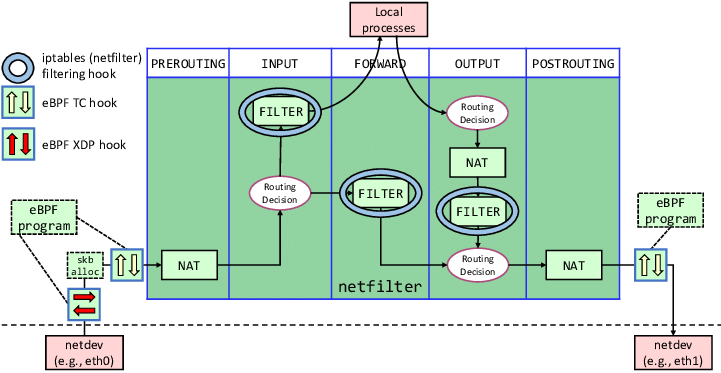
\includegraphics[width=\hsize]{images/mitigazione/hooks.png}
    \caption{Hooks eBPF}
    \centering
\end{figure}

\subsection{BPF Compiler Collection (BCC)}
 
È un framework che permette la scrittura di programmi python con programmi eBPF incorporati al loro interno. Il framework ha come obiettivo primario i casi in cui eBPF è utilizzata per raccogliere statistiche o compiere azioni in user space al verificarsi di eventi. L'esecuzione del programma eBPF genererà il bytecode che sarà caricato nel kernel \cite{ebpf.io}.
Il programma python potrà comunicare con quello eBPF grazie all'utilizzo delle mappe precedentemente menzionate.

\begin{figure}[]
    % todo: capire come gestire citazioni imsmagini a livello di copyright
    %  e capire come funzionano le label per richiamare le immagini
    \label{fig:bcc}
    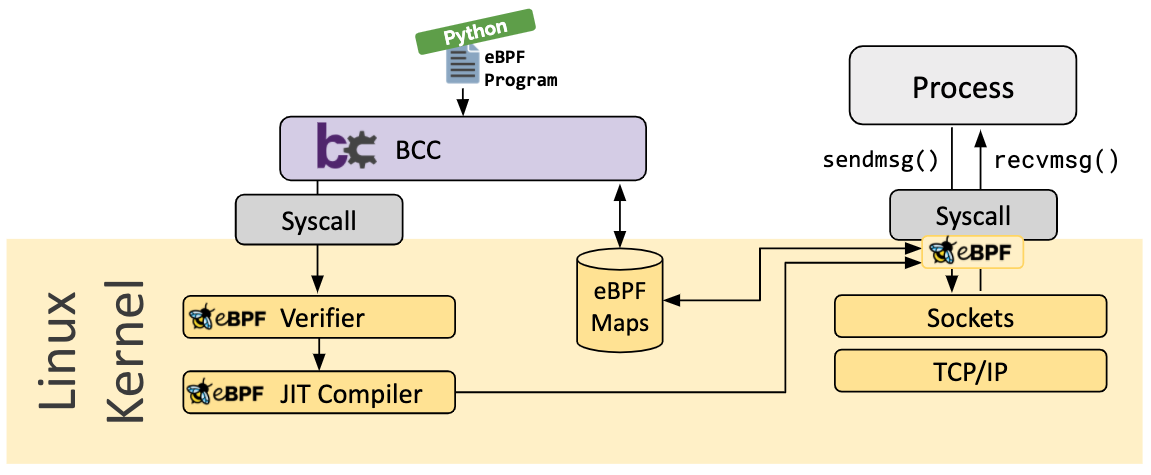
\includegraphics[width=\hsize]{images/mitigazione/bcc.png}
    \caption{Funzionamento di BCC \cite{ebpf.io}}
    \centering
\end{figure}

\section{Funzionamento}

Qua posso parlare di due alternative, la prima è riutilizzare il sistema di anomaly detection simile a quello presentato precedentemente elencando tutti i problemi e i vantaggi.

%todo: citare articoli che usano netflow per rilevare le anomalie

Il secondo consiste nel raccogliere i dati come prima, e creare un ranking per ogni feature risultata anomala precedentemente e a quel punto blocco i flussi sopra una certa soglia, ma quale?

Mentre per l'ip spoofing come la gestisco?

\section{Test sulle anomalie}
\subsection{Tool utilizzati}
\subsection{Risultati}
